\section{Evaluation}
\label{sec:evaluation}

\subsection{Hypotheses}
The primary hypothesis is that the motion of speckle patterns can be effectively visualized using a photodiode array. 
Additionally, it is hypothesized that the use of multiple lasers will influence the signal-to-noise ratio (SNR) of the measurements.

\subsection{Apparatus}

The custom-designed PCB transmitted its analog signals to an 8-channel Digilent ADC MCC 128 DAQ Hat, which was powered by a 5V low-noise bench power supply. 
A piezo disc, positioned at a distance of approximately 30~cm, was excited using a signal generator set to produce a sine wave at 133~Hz with a peak-to-peak amplitude of 3~V. 

For visual alignment of the lasers, one camera was employed, while another camera was used to monitor the presence of speckles. 
Both the cameras and the photodiode array were equipped with 8~$\times$~8~$\times$~1~mm bandpass filters at 850~nm with a 40~nm FWHM and a 90\% transmission rate (manufacturer: Haian Subei Optical Glass Factory).
Data acquisition was handled by a Raspberry Pi, which recorded the ADC data. 
Data processing was performed in real time during qualitative experiments or recorded for later post-processing.

\subsection{Procedure}

The initial steps of the evaluation involved SPICE simulations to analyze the Bode plot and transient response of the amplifier, as illustrated in Figure \ref{fig:bodeplot}.

Noise simulations (TI TINA SPICE with models from Texas Instruments \ref{fig:spice}) predicted the SNR to be 81.6~dB for an output value of approximately 80~mV (corresponding to a 1~nA photocurrent at 1000~kHz). 
The transient response showed quick settling and no ringing.
This demonstrates that the amplifier displayed stable behavior with high gain and SNR. Based on these results, the PCB was layouted, ordered and assembled.

Following the PCB assembly, it was cleaned using isopropyl alcohol (IPA) and compressed air, particularly under the pads of the amplifier section. 
Removing all flux residue from the PCB was deemed critical to ensure stable operation. 
All measurements were conducted in a light-controlled environment to minimize interference from external light sources.

To assess the performance of the amplifier qualitatively, a single IR laser was used first. 
It was aimed at a painted wooden surface while tapping the surface, jumping on the floor or banging the room door shut. 

Next, a single laser was aimed at a vibrating piezo disc and the FFT of the 1d signal calculated.

To assess the influence of multiple laser sources, the piezo disc (at 133~Hz) was measured,
while lasers in the square array were activated incrementally (Figure~\ref{fig:lasers}). 

\begin{figure*}[t]
    \centering
    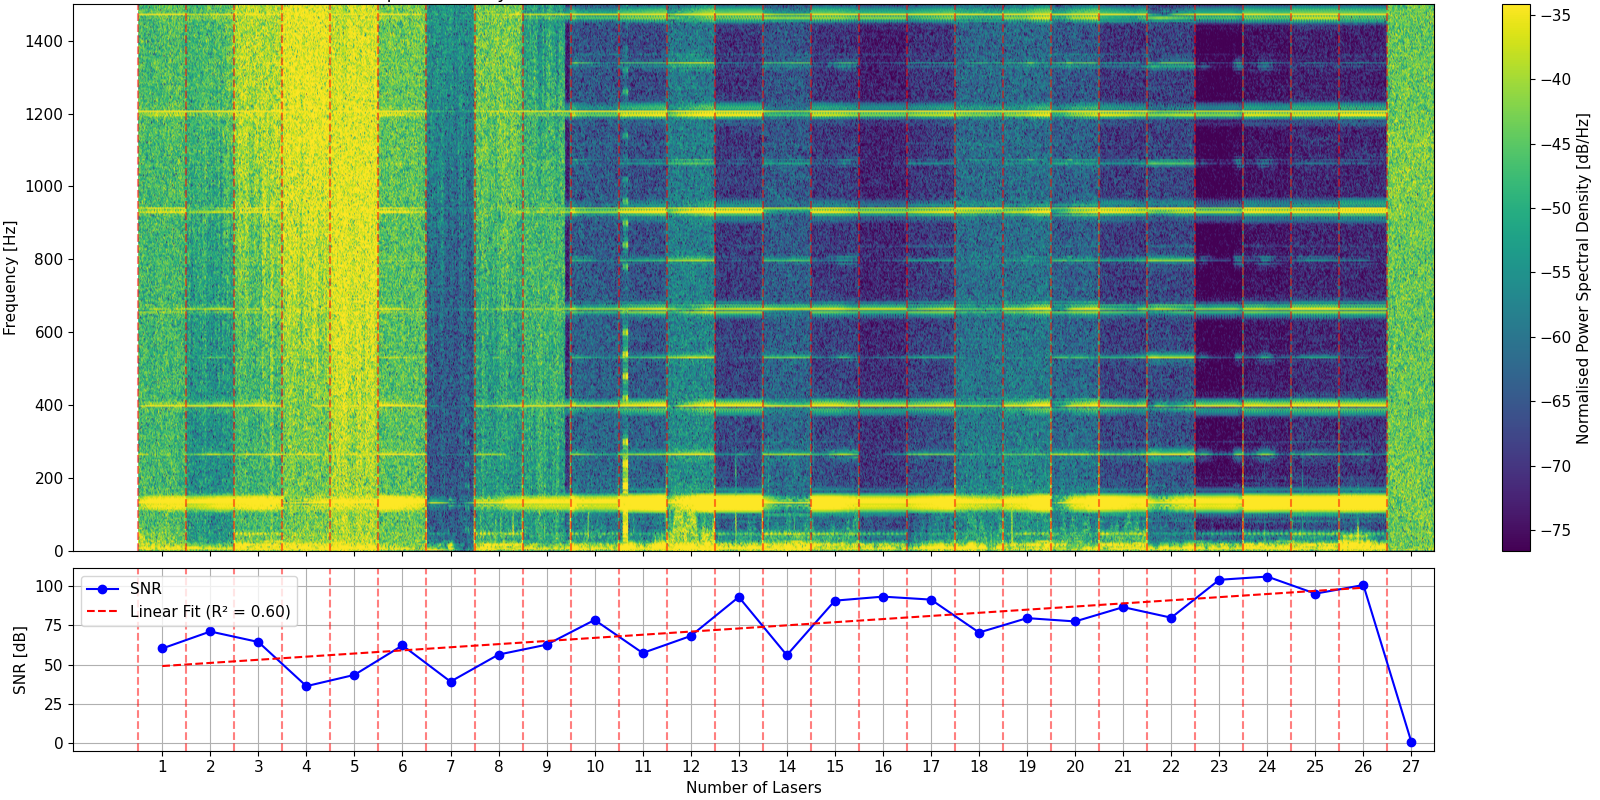
\includegraphics[width=\textwidth]{figures/results/multilaser_spectrogram.png}
    \caption{Spectral analysis of a 133~Hz surface vibration under different laser configurations. 
    Top: Power spectral density showing the target frequency component. Bottom: SNR improvement with increasing number of active lasers.}
    \label{fig:laser_snr}
\end{figure*}

For each configuration, the power spectral density of the inter-channel variance signal was calculated, and the SNR was analyzed. 
The spectral analysis, shown in Figure~\ref{fig:laser_snr}, 
established a positive correlation ($R^2 = 0.60$) between the number of active lasers and the detection SNR. 
A control measurement with all lasers switched off confirmed that the recorded signals originated from laser speckle patterns.

Additionally, time-domain signals captured by multiple photodiodes were compared to verify that each photodiode detected phase-shifted signals, which indicated the presence of a moving speckle pattern. 
An infrared (IR) LED was integrated into the setup to validate that the observed vibrations were dependent on coherent light.

\begin{figure}[t]
\centering
\includegraphics[width=\widthnarrow]{figures/eval/bode.png}
\caption{Amplifier frequency and phase response.}
\label{fig:bodeplot}
\end{figure}

% \begin{figure}[t]
% \centering
% 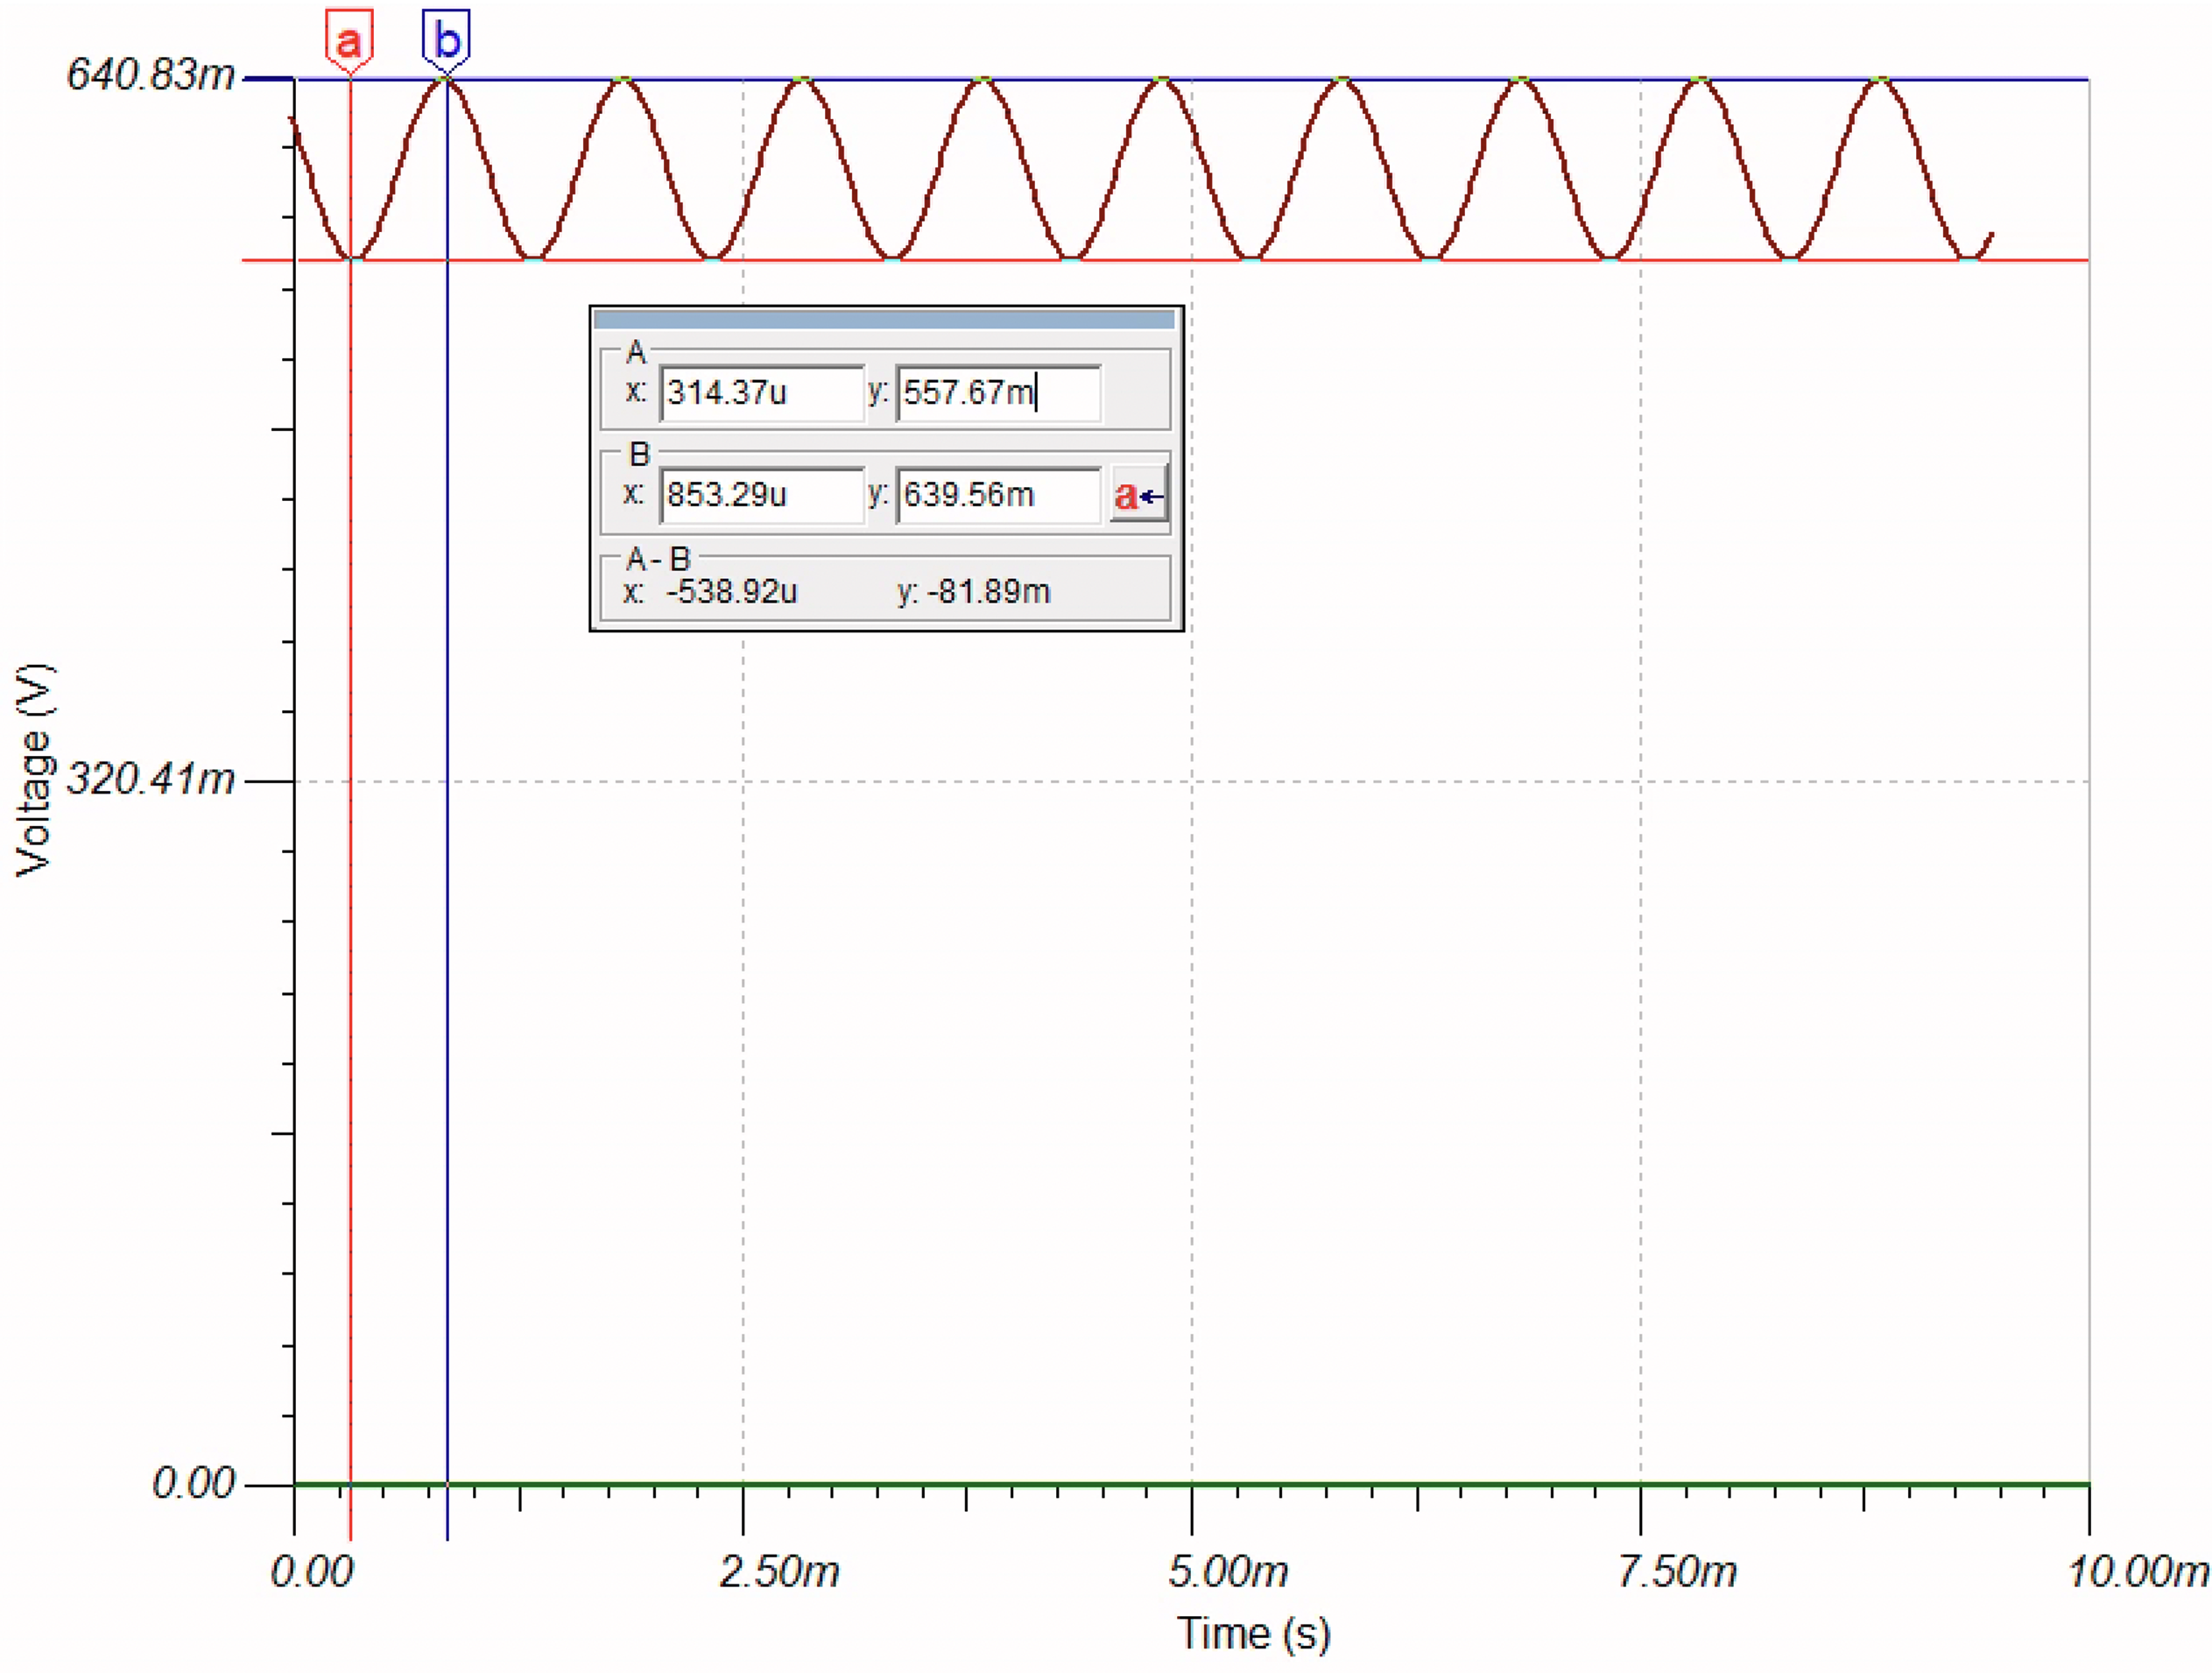
\includegraphics[width=\widthnarrow]{figures/eval/transient}
% \caption{Transient response captured during SPICE simulation, highlighting amplifier dynamics and stability.}
% \label{fig:transient}
% \end{figure}

% \begin{figure}[t]
% \centering
% 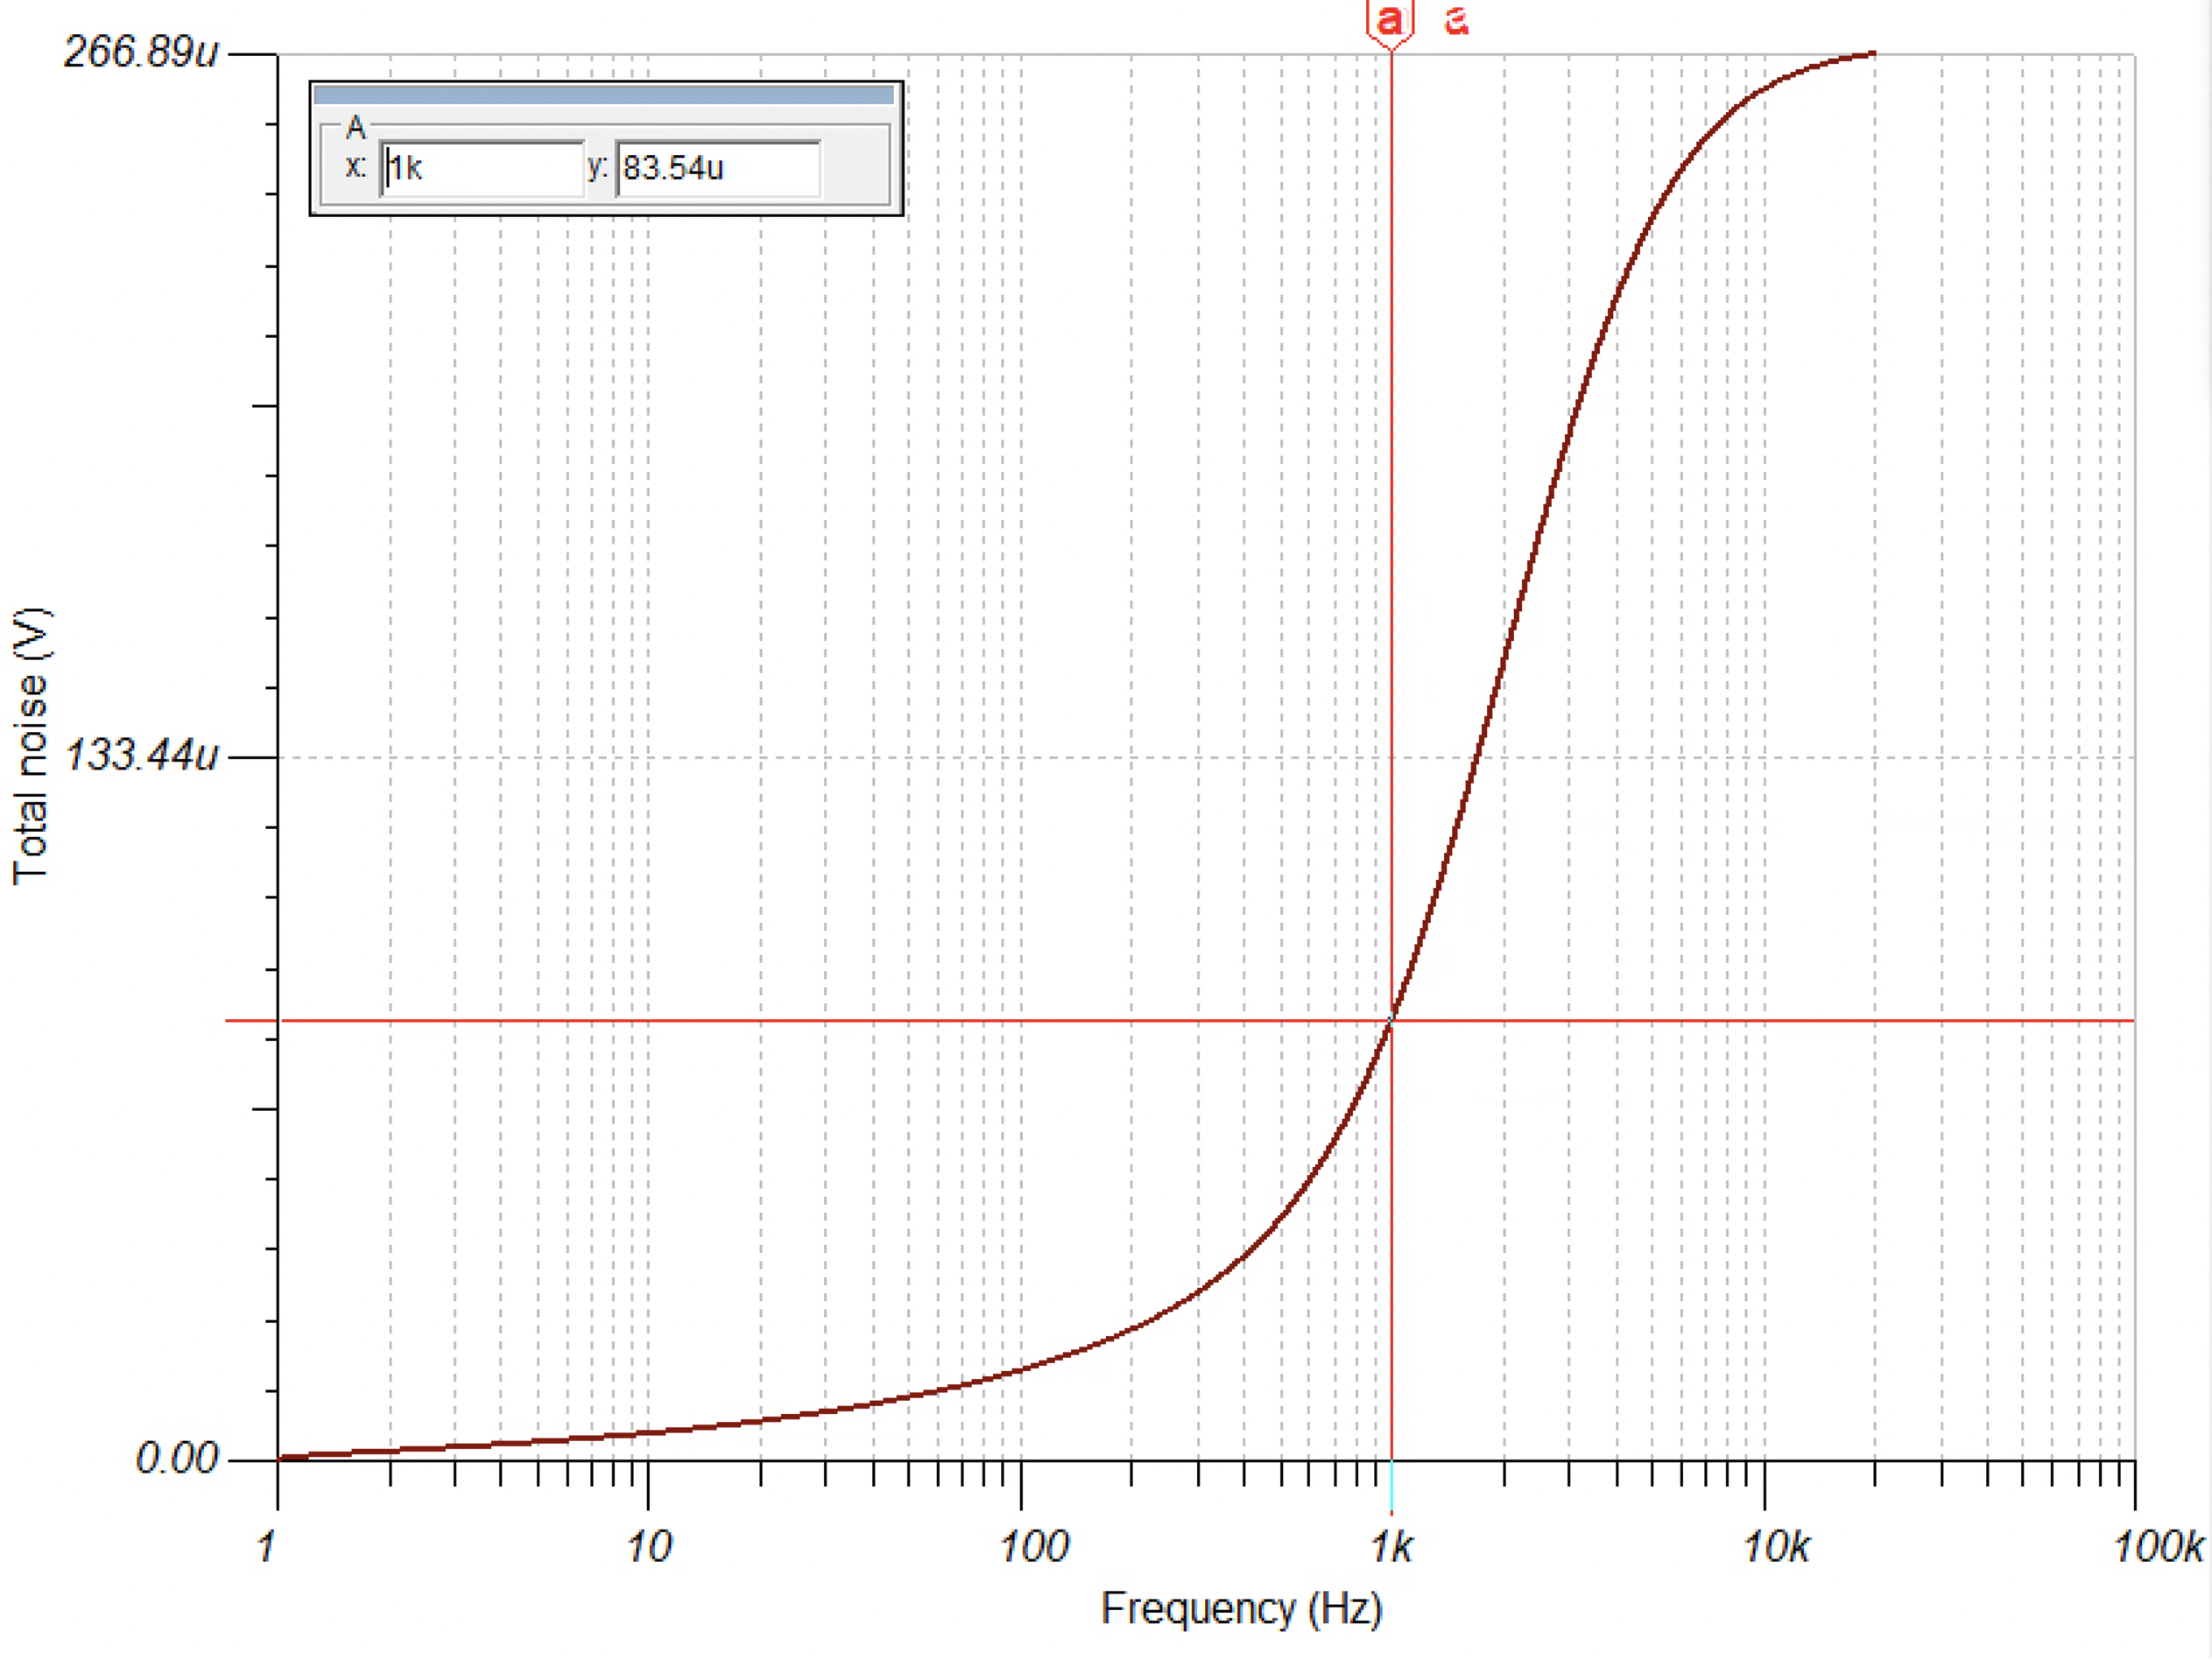
\includegraphics[width=\widthnarrow]{figures/eval/totalnoise.png}
% \caption{Total noise of the amplifier vs frequency.}
% \label{fig:totalnoise}
% \end{figure}

% \begin{figure}[t]
% \centering
% 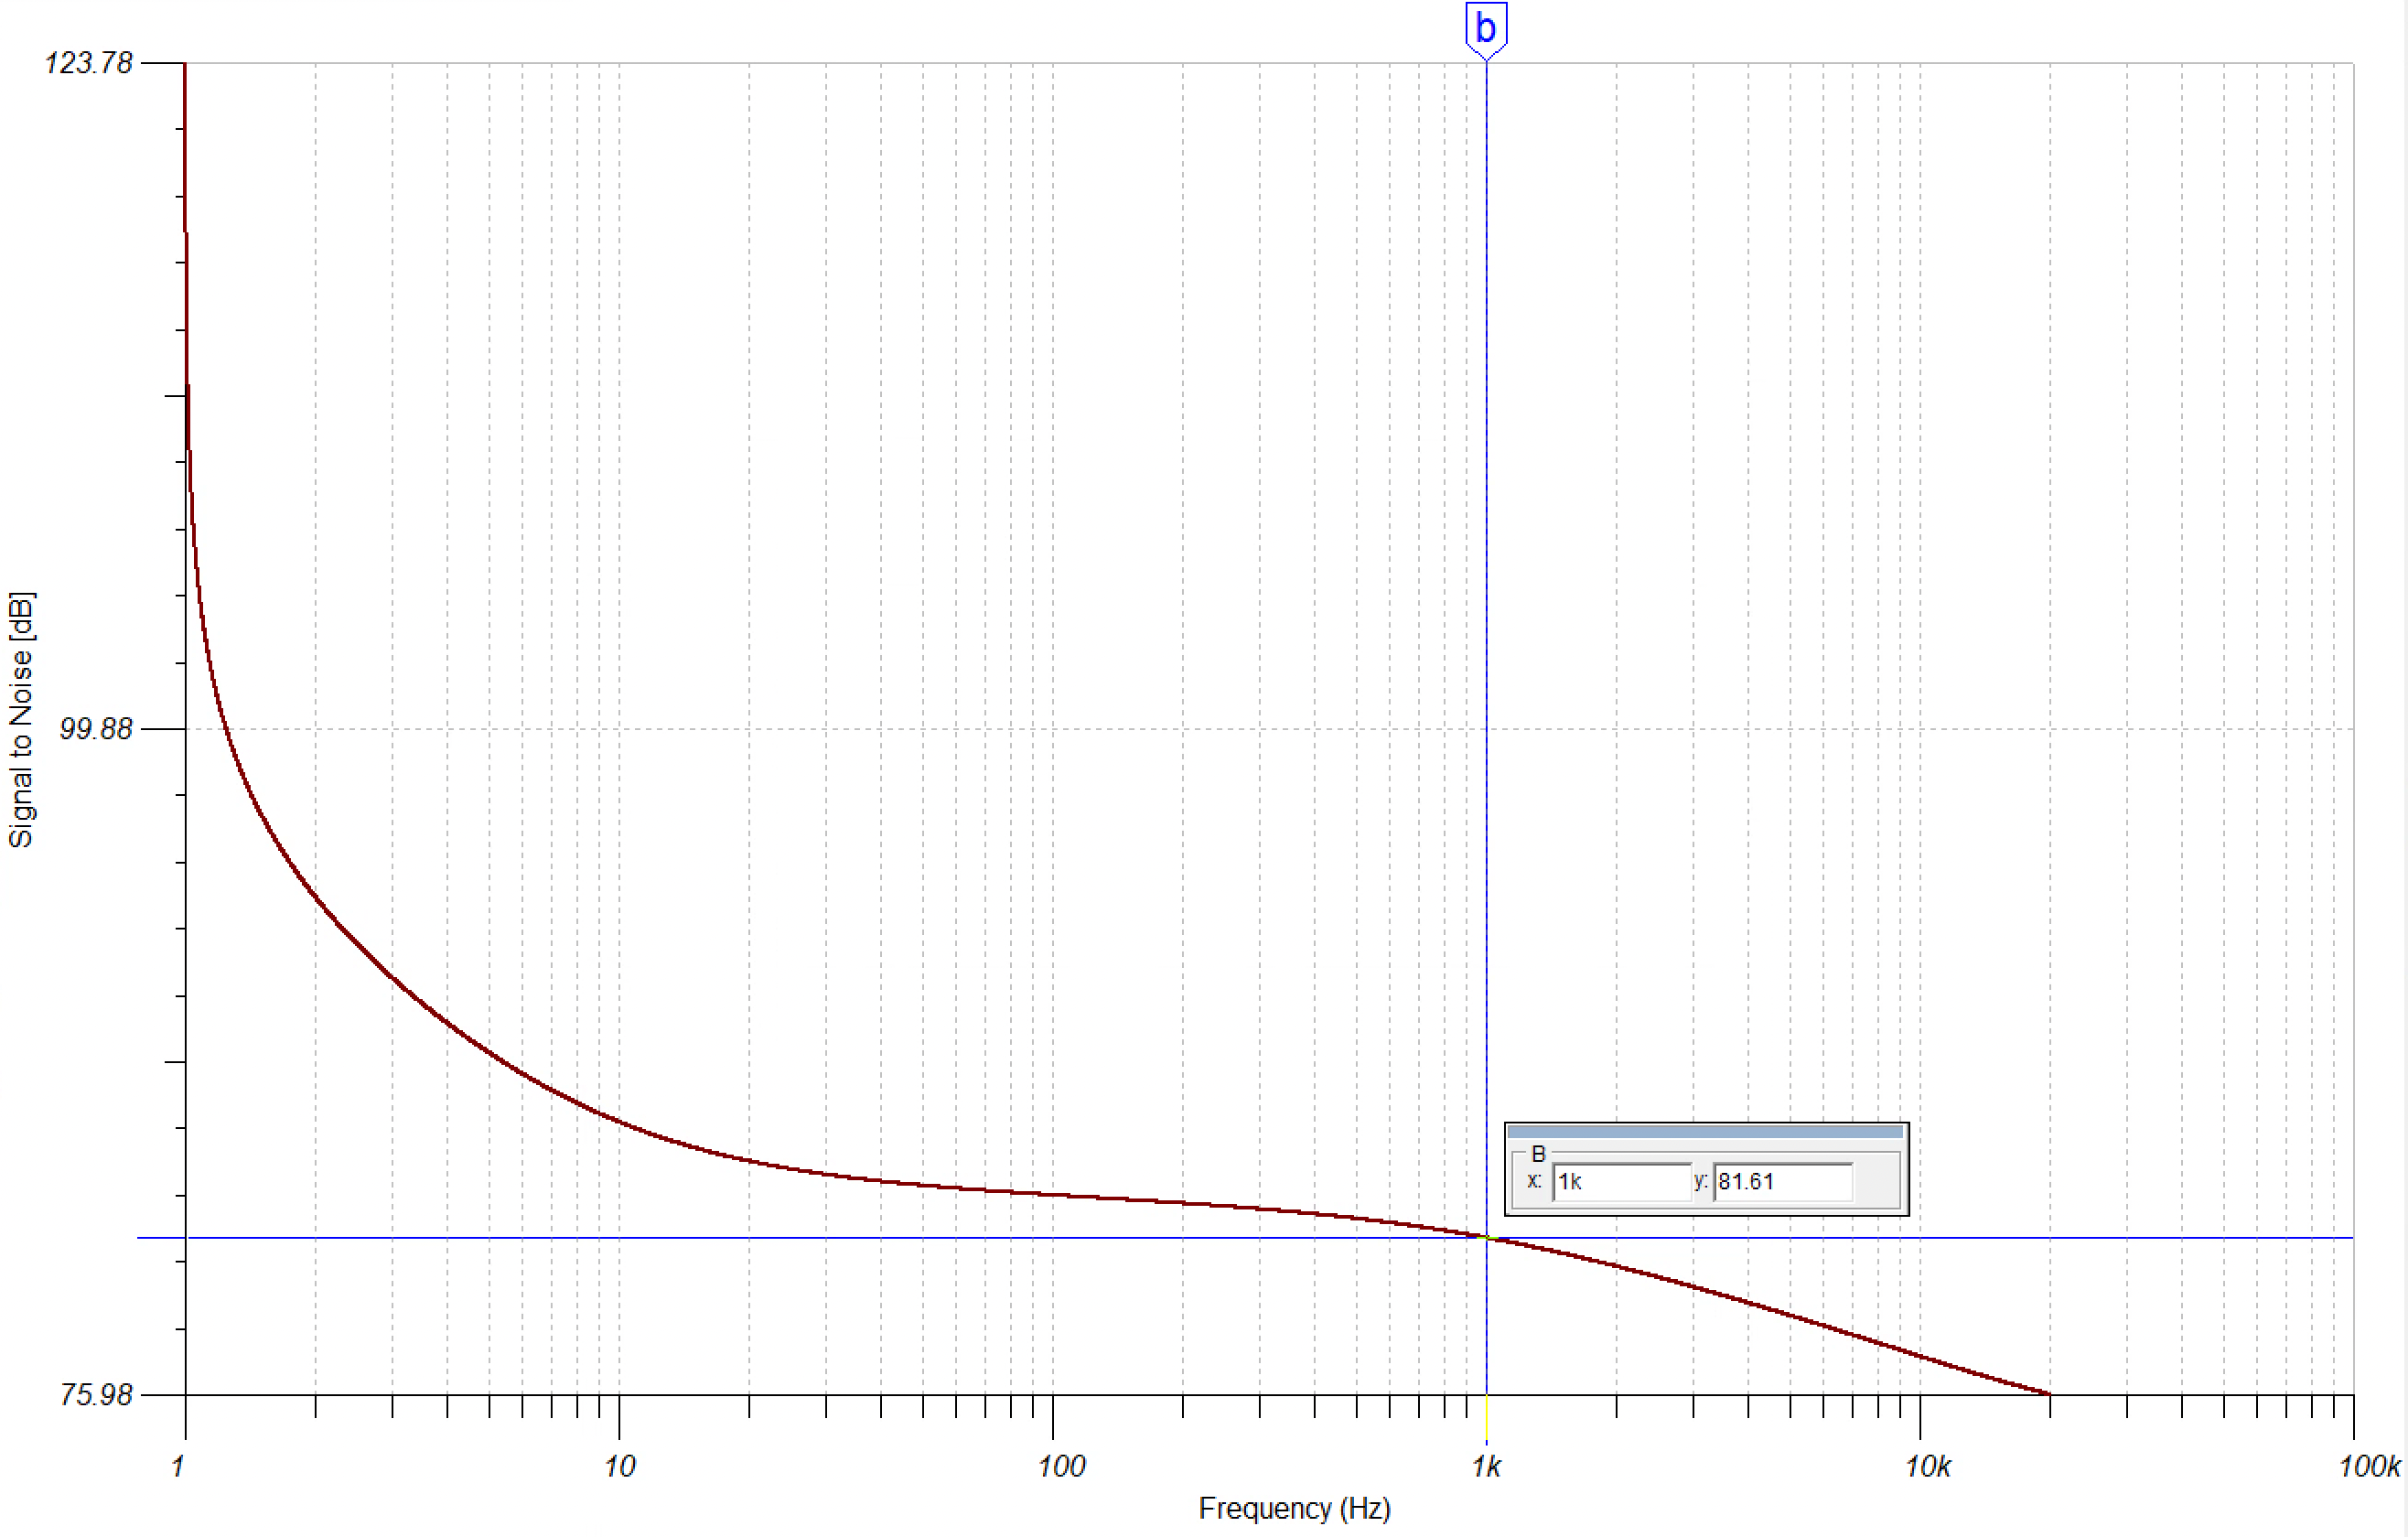
\includegraphics[width=\widthnarrow]{figures/eval/snr.png}
% \caption{SNR for an output value of approximately 80~mV (corresponding to a 1~nA photocurrent at 1000~kHz).}
% \label{fig:snr}
% \end{figure}